
% This LaTeX was auto-generated from an M-file by MATLAB.
% To make changes, update the M-file and republish this document.

\documentclass{article}
\usepackage{graphicx}
\usepackage{color}
\usepackage{listings}
\usepackage[framed]{mcode}
\usepackage{fullpage}
\usepackage{amsmath}
\usepackage[utf8x]{inputenc}
\usepackage{import}
\usepackage{setspace}
\usepackage{hyperref}
\definecolor{lightgray}{gray}{0.5}
\setlength{\parindent}{0pt}

\begin{document}

    
    
%\section*{}


\title{BE 521: Homework 5 \\{\normalsize Vision} \\{\normalsize Spring 2021}}
\author{42 points}
\date{Due: Tuesday, 03/02/2021 10 pm}
\maketitle \textbf{Objective:} Visual responses and likelihood


\begin{center} \author{Saif Khawaja \\
  \normalsize Collaborators: Raveen K \\}
\end{center}


\subsection*{V1 Dataset}
In this homework, you will work with data from 18 cells recorded from mouse primary visual cortex (also known as V1). Cells in this area are responsive to specific angles. Hence, a common stimulation paradigm is to show the subject a sinusoidal grating drifting at a specific angle (see Figure 1).
\begin{figure}[h!]
 \centering
 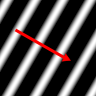
\includegraphics[width=48px]{figs/grad30.png}
 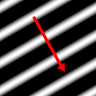
\includegraphics[width=48px]{figs/grad60.png}
 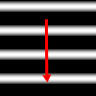
\includegraphics[width=48px]{figs/grad90.png}
 \caption{Example sinusoidal drifting grating at (in order left to right) 30, 60, and 90 degrees, where the red arrows shows the direction of the drift.}
\end{figure}
This data was collected and graciously provided by Daniel Denman in the Contreras Lab, University of Pennsylvania. The file \verb|mouseV1.mat| contains two variables: \verb|neurons|, a cell array representing all the times that each of the 18 cells fired a spike during the approximately 7 minute long experiment, and \verb|stimuli|, which provides the time (first column, in milliseconds) that a given angle (second column) was presented in this experiment.  Note that each stimulus in \verb|stimuli| is presented for exactly 2 seconds, after which a gray screen is presented for approximately 1.5 seconds (therefore each trial is approximately 3.5 seconds in duration.)
\section{Stimulus Response (11 pts)}
In this section, you will explore the response of the cells to different stimulus angles.
\begin{enumerate}
 \item How many unique grating angles, \textit{m}, are there in \verb|stimuli|? (1 pt)

\begin{lstlisting}
load("mouseV1.mat")
num_angles = length(unique(stimuli(:,2)))
\end{lstlisting}

\color{lightgray} \begin{lstlisting}
num_angles =

    12

\end{lstlisting} \color{black}

 \item A \emph{tuning curve} is frequently used to study the response of a neuron to a given range of input stimuli. To create tuning curves for this data, calculate the average number of spikes each cell fires in response to each grating angle. Store the result in an $18\times m$ dimensional matrix, where each element represents the response of a single neuron to a particular input stimulus angle, with each neuron assigned a row and each angle assigned a column. In a $2\times 2$ Matlab subplot, plot the tuning curve for the first four cells.  Place the stimulus angle on the x-axis and the number of spikes on the y-axis.  (6 pts)

\begin{lstlisting}
sorted = cell(num_angles,1);
labels = unique(stimuli(:,2));

for i = 1:num_angles
    sorted{i} = stimuli(stimuli(:, 2) == (i-1) * 30, 1);
end

spikes = zeros(18,num_angles);

for theta = 1:num_angles
    for stim_t = 1:length(sorted{theta})
        for ncounter = 1:length(neurons)
            for nactivity = 1:length(neurons{ncounter})
                if neurons{ncounter}(nactivity) >= sorted{theta}(stim_t) & neurons{ncounter}(nactivity) <= (sorted{theta}(stim_t) + 3.5e3)

                    spikes(ncounter, theta) = spikes(ncounter, theta) + 1;

                end
            end
        end
    end
end

tuningCurve = spikes/length(sorted{1});

figure
for i = 1:4
    subplot(2, 2, i)
    plot(0:30:330,tuningCurve(i,:),"LineWidth",1.125)
    xlim([0 360])
    title(sprintf("Neuron %d",i))
    ylabel("Average Spikes (#)")
    xlabel("Angle (o)")
end
sgtitle('Tuning Curves')
\end{lstlisting}


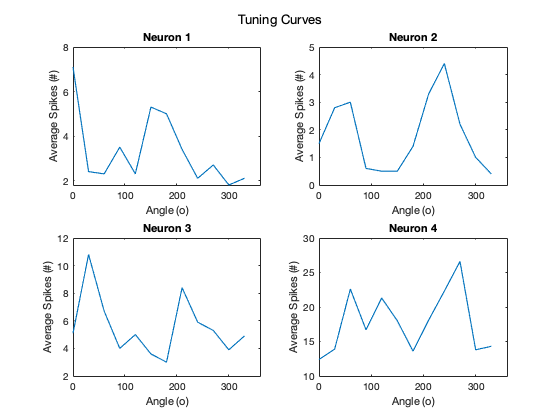
\includegraphics [width=5in]{HW5_Questions_01.png}

  \begin{enumerate}
   \item Look through the tuning response curves of each of the 18 cells.  How reasonable is it to assume that the response of a given cell to angle $\theta$ is the same as its response to angle $\theta+180$? Include at least a few tuning curves to back up your answer. (2 pts)

\begin{lstlisting}
randang = randperm(num_angles / 2, 3);

for i = 1:3
    figure
    subplot(2, 1, 1)
    plot(1:18, tuningCurve(:,randang(i)),"LineWidth",1.25)
    xlim([1 18])
    title(sprintf("Tuning Curve across Neurons %d degrees", labels(randang(i))))
    ylabel("Average Spikes (#)")
    xlabel("Angle (o)")
    subplot(2,1,2)
    plot(1:18, tuningCurve(:, randang(i) + 6),"LineWidth",1.125)
    xlim([1 18])
    title(sprintf("Tuning Curve %d degrees", labels(randang(i)+6)))
    ylabel("Average Spikes (#)")
    xlabel("Angle (o)")
end
\end{lstlisting}


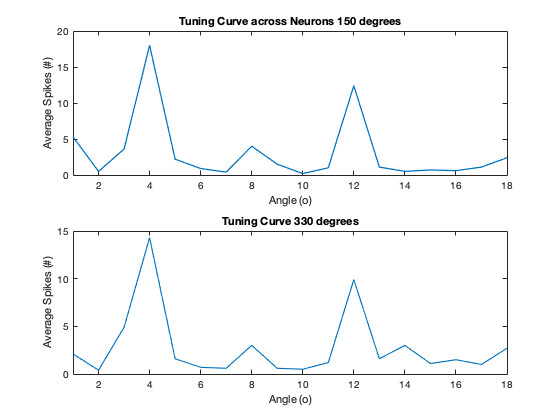
\includegraphics [width=5in]{HW5_Questions_02.png}


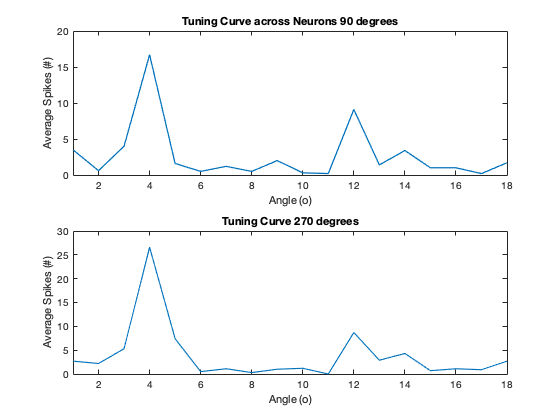
\includegraphics [width=5in]{HW5_Questions_03.png}


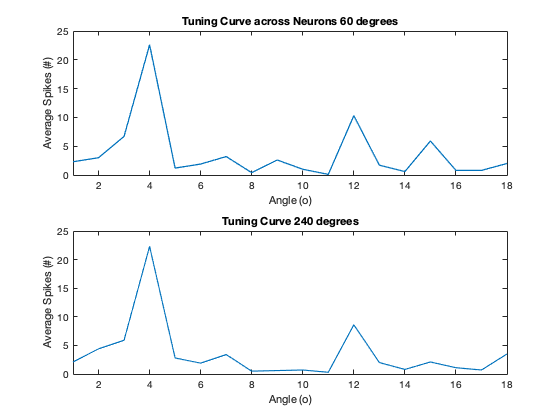
\includegraphics [width=5in]{HW5_Questions_04.png}

   \item Does this assumption have any physiological justification (given what you know about the types of cells in V1)? (2 pts)

\begin{lstlisting}
% Given that the V1 cells process visual information and that the grating
% permits certain angles through, one would see the same stimuli as the
% grating is similarly aligned. We can expect the responses should be identical
% at both angles and therefore the assumption is reasonable. There is some
% variation here, however, but we can speculate this is do to minor physiological
% differences between cells.
\end{lstlisting}

  \end{enumerate}
\end{enumerate}
\section{Neural Decoding (31 pts)}
Suppose we would like to work backwards - that is, for a given neural response, can we predict what the grating angle was? This process is called ``neural decoding,'' and is especially of interest to the BCI motor control community (as we'll see in a later homework).
In this section, we will try out an approach which is detailed in Jazayeri \& Movshon 2006 \footnote{A copy of this paper is included if you are curious, but we walk you through the method in this homework.}.
The method we will use involves finding the maximum likelihood of
the data. \\ \\
Here, the data is the number of spikes $s_i$ that cell $i$ fires when the subject sees a stimulus with grating angle $\theta$. One way to think about our likelihood function is to ask the question ``given a stimulus angle $\theta$, how many spikes would I expect this cell to fire?'' We can represent this number of spikes $s_i$ using a Poisson process with parameter $f_i(\theta)$ for a stimulus $\theta$, where $f_i$ represents neuron $i$'s tuning function.
A Poisson distribution is often used to model count data that occurs at a constant rate, and in this case the rate is given by $f_i(\theta)$. In other words, our likelihood function $L_i(\theta)$ for each neuron $i$ is the probability $p(s_i|\theta)$ of neuron $i$ firing $s_i$ spikes for a given value of $\theta$.
The idea in this method is to calculate the log likelihood\footnote{log = natural log unless otherwise specified} function of each neuron and then add them all together to get the log likelihood function of the entire population of ($n$) neurons. We often work with the $\emph{log}$ likelihood because it allows adding of probabilities instead of multiplying, which can lead to numerical problems.
\begin{align*}
p(s_i|\theta) \sim &\; Pois(f_i(\theta)) = \frac{f_i(\theta)^{s_i}}{s_i!} e^{-{f_i(\theta)}} \tag{Poisson probability density}\\
\L_i(\theta) =&\; p(s_i|\theta) \tag{Likelihood of a given neuron firing at $s_i$}\\
\L(\theta) = &\; \prod_{i=1}^n p(s_i|\theta) \tag{Joint likelihood of all n neurons}\\
\log \L(\theta) = &\;\sum_{i=1}^n \log L_i(\theta) = \sum_{i=1}^n \log p(s_i|\theta)  \tag{Take log}\\
\propto &\;  \sum_{i=1}^n s_i \log f_i(\theta) \tag{evaluation of PDF and simplifying}
\end{align*}
Thus, we can define the log likelihood for each neuron $i$ as the log of its tuning curve $f_i(\theta)$ times the number of spikes $s_i$ it fires for a particular stimulus $\theta$, and the population log likelihood is simply the summation across all cells. This tells us that, given a set of tuning curves $f_i(\theta)$, we can compute the likelihood of observing our data $s$.
But we already have those tuning curves for each cell from question 1.2, so all we need to know for a new (hidden) stimulus is how many spikes each neuron fires. Let $\mathbf{s}$ be the $n$-dimensional column vector of the number of spikes each cell fires after the subject is presented with a new stimulus $\theta'$ and let $\mathbf{F}$ be the $n\times m$ matrix representing the tuning curves of each neuron at each of the $m$ stimuli (for us, $m$ is the number of stimuli between 0 and 150 degrees because we assume that all neurons respond equally to $\theta$ and $\theta+180$ degrees.)  We can then compute the log likelihood of the new stimulus $\theta'$ easily using the inner product of $\mathbf{s}$ and $\mathbf{F}$: \verb|L = s'*log(F)|.
\begin{enumerate}
 \item Compute the matrix \verb|F| by recalculating the tuning curves you calculated in question 1.2 using only the \textbf{first 70} trials (this is akin to our ``training'' data). You will use the remaining 50 trials (as ``testing'' data) to make predictions. Make a histogram of the number of stimulation angles for the first 70 trials to ensure that each angle (0 to 150) is presented at least a few times. (4 pts)

\begin{lstlisting}
angsorted = cell(6, 1);

anghist = zeros(70, 1);

startCount = 1;

for i = 1:num_angles / 2
    angsorted{i} = [stimuli(stimuli(1:70, 2) == (i - 1) * 30, 1);
    stimuli(stimuli(1:70, 2) == (((i - 1) * 30) + 180), 1)];
    totalAngles = length([stimuli(stimuli(1:70,2) == (i-1)*30,1);
    stimuli(stimuli(1:70,2) == (((i-1)*30) + 180),1)]);

    anghist(startCount:startCount + totalAngles - 1) = [stimuli(stimuli(1:70,2) == (i-1)*30,2); stimuli(stimuli(1:70,2) == (((i-1)*30) + 180),2) - 180];
    startCount = startCount + totalAngles;
end

F = zeros(18,num_angles/2);

spiketest = zeros(18,num_angles/2);

for theta = 1:num_angles/2
    for stim_t = 1:length(angsorted{theta})
        for ncounter = 1:length(neurons)
            for nactivity = 1:length(neurons{ncounter})
                if neurons{ncounter}(nactivity) >= angsorted{theta}(stim_t) & neurons{ncounter}(nactivity) <= (angsorted{theta}(stim_t) + 3.5e3)
                    spiketest(ncounter,theta) = spiketest(ncounter,theta) + 1;
                end
            end
        end
    end

F(:,theta) = spiketest(:,theta)/(length(angsorted{theta}));

end

figure
histogram(anghist,6)
xlabel("Angle (o)")
ylabel("Spikes (#)")
title("Distribution of first 70 sample angles")
\end{lstlisting}


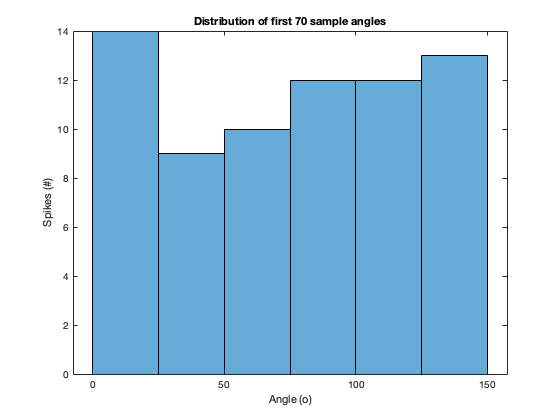
\includegraphics [width=5in]{HW5_Questions_05.png}

 \item For the 50 ``testing'' trials, compute a $n \times 50$ matrix \verb|S| where each row
represents the number of spikes one neuron fired in response to a each of the 50 trials. With this, you can easily compute the log likelihood functions for all the trials at
once with the command: \verb|L_test = S'*log(F)|. (Hint: add a small number to \verb|F| to avoid taking the log of 0)
  \begin{enumerate}
	\item Plot the likelihood functions for the first four testing trials in a $2\times 2$ subplot. In the title of each plot, give the trial number (1, 2, 3, or 4) and the true stimulation angle. Make sure to label your axes correctly. (5 pts)

\begin{lstlisting}
exp_ang = cell(6,1);

for i = 1:num_angles/2
    exp_ang{i} = [stimuli(stimuli(71:120,2) == (i - 1)*30,1);
        stimuli(stimuli(71:120,2) == (((i-1)*30) + 180),1)];
end

s = zeros(18,50);

for stim_t = 71:120
    for ncounter = 1:length(neurons)
        for nactivity = 1:length(neurons{ncounter})
            if neurons{ncounter}(nactivity) >= stimuli(stim_t,1) & neurons{ncounter}(nactivity) <= (stimuli(stim_t, 1) + 3.5e3)

                s(ncounter,stim_t - 70) = s(ncounter,stim_t - 70) + 1;

            end
        end
    end
end

L = s' * log(F);

figure
subplot(2, 2, 1)
plot(labels(1:6),L(1,:),'LineWidth',1.125)
xlabel("Angle (o)")
ylabel("Log Likelihood")
title(['Trial 1 | Stim Angle = ', num2str(stimuli(71,2)),' degrees'])
subplot(2,2,3)
plot(labels(1:6),L(3,:),'LineWidth',1.125)
xlabel("Angle (o)")
ylabel("Log Likelihood")
title(['Trial 3 | Stim Angle = ', num2str(stimuli(73,2)),' degrees'])
subplot(2, 2, 2)
plot(labels(1:6),L(2,:),'LineWidth',1.125)
xlabel("Angle (o)")
ylabel("Log Likelihood")
title(['Trial 2 | Stim Angle = ', num2str(stimuli(72,2)-180),' degrees'])
subplot(2,2,4)
plot(labels(1:6),L(4,:),'LineWidth',1.125)
xlabel("Angle (o)")
ylabel("Log Likelihood")
title(['Trial 4 | Stim Angle = ', num2str(stimuli(74,2)),' degrees'])
\end{lstlisting}


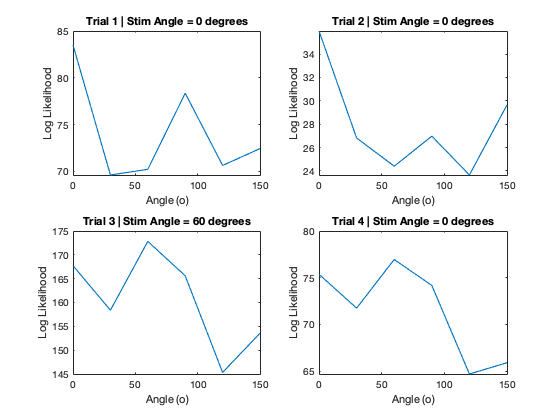
\includegraphics [width=5in]{HW5_Questions_06.png}

	\item How well do these four likelihood functions seem to match the true stimulation angle? Explain in a few sentences. (3 pts)

\begin{lstlisting}
% There is some success since they predicted 3/4 of the graphs as well as
% demonstrate peak likelihoods for 1, 2 and 3. 1 and 3 did have a high
% likelihood at other angles, so the functions are only marginally
% sufficient to determine given a sizeable error that independently might
% provide alternative conclusions.
\end{lstlisting}

	\item Compute the maximum likelihood estimate (MLE) for each of
	the 50 trials. This is another way of asking which angle $\theta$ has the highest probability.
	\[ \hat{\theta}_{MLE} = \arg\max_\theta\; L(\theta) = \arg\max_\theta\; \log L(\theta) \]
	In what percentage of the 50 trials did your MLE correctly predict the stimulation angle [0-150]? (5 pts)

\begin{lstlisting}
expang = zeros(50, 2);

for i = 1:50
    if stimuli(70 + i,2) >= 180
        expang(i,1) = stimuli(70 + i,2) - 180;
    else
        expang(i,1) = stimuli(70 + i,2);
    end
    [~, ColInd] = max(L(i,:));

    expang(i,2) = labels(ColInd);
end

Correct = (sum(expang(:,1) == expang(:,2)))/50*100

% 42% Accuracy
\end{lstlisting}

\color{lightgray} \begin{lstlisting}
Correct =

    42

\end{lstlisting} \color{black}

	\item
	In a few sentences, discuss how well this method worked for predicting the input angle from the response of the 18 neurons.  What might you change in the experimental protocol to try and get a better prediction? (3 pts)
	\end{enumerate}

\begin{lstlisting}
% We can see that, although 42% is not very accurate independently, this method
% performed better instead of random selection of angles. Gathering more data by
% conducting more trials would lead to more success in a
% Poisson-distributed system as there would be less sway in statistics by
% particular outlier values, which provides a better foundation for
% predictive capabilities. Adjustments to the process to use a greater
% number of nerons could also be more successful with the likelihood
% prediction using the whole population and more data provides more
% informatoin for a more representative conclusion.
\end{lstlisting}

  \item It is important to show that your findings are not a result of chance. One way to demonstrate this is using a ``permutation test.'' Here, we will perform a permutation test by randomly reassigning new grating angles to the 50 test responses and then calculating how often the new grating angles match the true stimulation angles.
	\begin{enumerate}
	 \item Simulate the chance prediction (the ``null'' distribution) by randomly reassigning the stimulation angles 1000 times.  For each permutation, calculate the percent accuracy of each label. Create a histogram of the 1000 accuracy measurements for the null distribution. Add a red vertical line with the accuracy calculated from using the Jazayeri method above. (4 pts)

\begin{lstlisting}
permt = zeros(50,2);

permt(:,2) = stimuli(71:120,2);

perma = zeros(1000,1);

permt(permt(:,2) >=180, 2) = permt(permt(:,2) >=180, 2) - 180;

for p = 1:1000

    random = randi(6,50,1);
    permt(:,1) = labels(random);

    Correct = sum(permt(:,1) == permt(:,2)); perma(p) = (Correct/50) * 100;
end

figure
hold on
histogram(perma)
xline(42,'r','LineWidth',1.125)
ylabel("Count (#)")
xlabel("Percentage Accuracy")
title("Null Distribution Histogram")
\end{lstlisting}


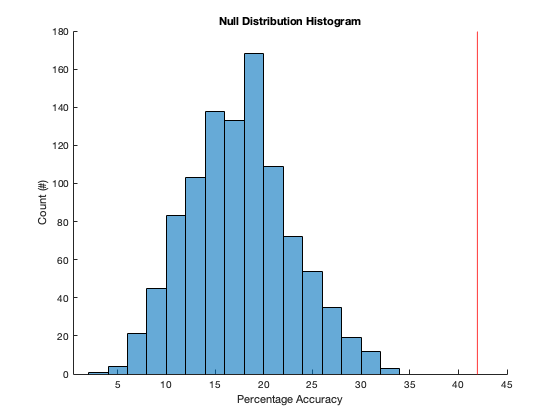
\includegraphics [width=5in]{HW5_Questions_07.png}

	 \item Is the null distribution what you expected? Explain. (1 pt)

\begin{lstlisting}
% With the approximate centering around 1/6 (16.67%), the Gaussian
% distribution is centered around the expectated value (1/6's bin has the
% highest count), and so we received an expected shape.
\end{lstlisting}

	\item What is the probability that your actual accuracy measurement comes from the null-distribution?  That is, calculate the fraction of permutation samples with accuracy \emph{more extreme} relative to the mean of the null distribution (less than your measurement if your value is less than the mean, or more than your measurement if your value is more than the mean). (2 pts)

\begin{lstlisting}
count = sum(perma >= 42);

pVal = (count/1000) * 100
\end{lstlisting}

\color{lightgray} \begin{lstlisting}
pVal =

     0

\end{lstlisting} \color{black}

	\item What would the probability be if your accuracy had been 25\%? (1 pt)

\begin{lstlisting}
count = sum(perma >= 25);

pVal = (count/1000) * 100
\end{lstlisting}

\color{lightgray} \begin{lstlisting}
pVal =

    6.9000

\end{lstlisting} \color{black}

	\item What is this value typically called? (1 pt)

The p-value.

	\end{enumerate}
  \item The tuning curves and neuron responses to a new trial were calculated using the number of spikes each neuron fired after the stimulation. But what if a particular neuron just happens to fire a lot and fires even more when it gets a stimulus to which it's tuned? Those neurons could ``swamp'' the log likelihood estimate given in Equation 1 by virtue of just having a larger average $s_i$ and $f_i(\theta)$.
  How might we correct for this type of behavior?  Suggest a possible method. (2 pts)

\begin{lstlisting}
% Before we perform calculations with si and fi(θ), we could average each
% to neuron to itself with say individual fire counts and max firing coutns
% to normalize the activity to each neuron (and particular values will not
% skew the distribution).
\end{lstlisting}

\end{enumerate}
\end{document}




\end{document}
    
